% This is "sig-alternate.tex" V2.0 May 2012
% This file should be compiled with V2.5 of "sig-alternate.cls" May 2012
%
% This example file demonstrates the use of the 'sig-alternate.cls'
% V2.5 LaTeX2e document class file. It is for those submitting
% articles to ACM Conference Proceedings WHO DO NOT WISH TO
% STRICTLY ADHERE TO THE SIGS (PUBS-BOARD-ENDORSED) STYLE.
% The 'sig-alternate.cls' file will produce a similar-looking,
% albeit, 'tighter' paper resulting in, invariably, fewer pages.
%
% ----------------------------------------------------------------------------------------------------------------
% This .tex file (and associated .cls V2.5) produces:
%       1) The Permission Statement
%       2) The Conference (location) Info information
%       3) The Copyright Line with ACM data
%       4) NO page numbers
%
% as against the acm_proc_article-sp.cls file which
% DOES NOT produce 1) thru' 3) above.
%
% Using 'sig-alternate.cls' you have control, however, from within
% the source .tex file, over both the CopyrightYear
% (defaulted to 200X) and the ACM Copyright Data
% (defaulted to X-XXXXX-XX-X/XX/XX).
% e.g.
% \CopyrightYear{2007} will cause 2007 to appear in the copyright line.
% \crdata{0-12345-67-8/90/12} will cause 0-12345-67-8/90/12 to appear in the copyright line.
%
% ---------------------------------------------------------------------------------------------------------------
% This .tex source is an example which *does* use
% the .bib file (from which the .bbl file % is produced).
% REMEMBER HOWEVER: After having produced the .bbl file,
% and prior to final submission, you *NEED* to 'insert'
% your .bbl file into your source .tex file so as to provide
% ONE 'self-contained' source file.
%
% ================= IF YOU HAVE QUESTIONS =======================
% Questions regarding the SIGS styles, SIGS policies and
% procedures, Conferences etc. should be sent to
% Adrienne Griscti (griscti@acm.org)
%
% Technical questions _only_ to
% Gerald Murray (murray@hq.acm.org)
% ===============================================================
%
% For tracking purposes - this is V2.0 - May 2012

%\documentclass{acm_proc_article-sp}
\documentclass{sig-alternate}
\usepackage{color}
\usepackage{multirow}
\usepackage{listings}
\usepackage{url}

\lstset{language=java, numbers=left, numberstyle=\tiny\color{black}, numbersep=3pt, escapeinside={\$}, basicstyle=\footnotesize\ttfamily, escapeinside={\%*}{*)}}

\newif\ifdraft
\drafttrue
%\draftfalse                                                                              
\ifdraft
\newcommand{\zhaonote}[1]{{\textcolor{cyan}    { ***Zhao:      #1 }}}
\newcommand{\evannote}[1]{{\textcolor{red}    { ***Evan:      #1 }}}
\newcommand{\note}[1]{ {\textcolor{red}    {\bf #1 }}}
\else
\newcommand{\zhaonote}[1]{}
\newcommand{\evannote}[1]{}
\newcommand{\note}[1]{}
\fi

\newenvironment{shortlist}{
        \vspace*{-0.5em}
  \begin{itemize}
  \setlength{\itemsep}{-0.1em}
}{
  \end{itemize}
        \vspace*{-0.5em}
}

\begin{document}

\title{Gineala: Debugging Machine Learning Pipelines with Fine-grained Lineage}

\numberofauthors{3} 
\author{
% 1st. author
\alignauthor Zhao~Zhang\\\
       \affaddr{AMPLab}\\
       \affaddr{University of California, Berkeley} \\
       \email{zhangzhao@berkeley.edu}    
% 4th. author       
\alignauthor Evan~R.~Sparks\\\
       \affaddr{AMPLab}\\
       \affaddr{University of California, Berkeley}\\
       \email{sparks@cs.berkeley.edu}       
% 6th. author
\alignauthor Michael~J.~Franklin\\
       \affaddr{AMPLab}\\
       \affaddr{University of California, Berkeley}\\
       \email{franklin@berkeley.edu}   
}

\maketitle

\begin{abstract}
Distributed machine learning (ML) frameworks are increasingly popular as practitioners and researchers 
can quickly build productive applications (ML pipelines) and execute them at scale. 
Debugging such a pipeline is often cumbersome due to the lack of system support for
recording intermediate state and user interaction.
In this paper, we explore the debuggability issue of distributed ML systems by leveraging fine-grained 
data lineage throughout ML pipelines. 
Specifically, we formulate the fine-grained data lineage as mappings between multi-dimensional spaces,
identify a suite of primitive lineage types based on its mapping patterns, 
and investigate several recording and indexing strategies to reduce the storage consumption and improve the query performance.

We present the Gineala lineage system and integrate it with KeystoneML, a distributed machine learning
application framework built on top of Apache Spark. 
Gineala exposes an API derived from \emph{primitive lineage types} and collects fine-grained data lineage for each 
data transformation by recording the input datasets, the output datasets and the mapping between them along
with all information needed to reproduce the computation - including program logic, model parameters, and random seed values.
Gineala efficiently enables data anomaly removal and computation replay, code debugging, and result analysis.
Practically, the Gineala can reduce the storage consumption by up to 45x and speeds up the query performance
by up to 31x. The performance penalty introduce by Gineala is 16\%-54\% depending on the pipeline and
use case.

\end{abstract}

% A category with the (minimum) three required fields
\category{Scalable Data Analysis}{System for Data Management}[Big Data]
%\keywords{ACM proceedings, \LaTeX, text tagging}

\section{Introduction}
Machine learning frameworks are increasingly popular as practitioners and researchers can quickly
build productive applications (referred to as ML pipelines in the rest of this paper) with a high-level 
programming language to pipeline data preparation, feature extraction, model training, 
and prediction. 
Among these systems, Scikit-learn~\cite{pedregosa2011scikit} and TensorFlow~\cite{tensorflow15} \evannote{tensorflow is distributed}
are single-computer-based framework while Apache Mahout~\cite{owen2011mahout}, MLlib~\cite{meng2015mllib}, 
SystemML~\cite{ghoting11systemml}, and KeystoneML~\cite{sparks15} focus on a distributed environment.

Debugging such an ML pipeline with datasets in a distributed environment can be problematic due to
the lack of system support of memory states capturing and user interaction.
To motivate, we present three typical use cases for ML pipeline debugging:
\begin{shortlist}
\item{\bf Data Debugging}: In a hand-written digit classification pipeline, a user wants to remove one
corrupted training data item and retrain the model.
\item{\bf Code Debugging}: In an image classification pipeline, a user wants to verify the correctness of 
the positional information of features. 
\item{\bf Results Debugging}: In an astronomical object extraction pipeline, an astronomer wants to find objects whose
brightness are above a threshold then locate them in the input images.
\end{shortlist}

In practice, users instrument the steps of interest to gather intermediate state and store it in persistent storage
for later examination. Users may try multiple solutions until this state contains sufficient information to support the
use case. These solutions are often use case specific, performance degradation prone, and can complicate code
management due to the demand for multiple versions of a pipeline.
\evannotes{Given that this is a repeated pattern taken on by users of the system, it is natural to add fully automated support that is transparent to users in terms of performance and application complexity..}

On the other hand, fine-grained data lineage at data structure cell-level (e.g. elements of a matrix) -- the mapping between
input elements to output elements and according computation -- can provide useful information for
debugging~\cite{widom04}. The user of the {\bf Data Debugging} case can trace the propagation of the corrupted training
data item from the beginning step forward until the step before model training to figure out the affected features.
Then the user traces the affected features backward and confirms these affected features only depend on the corrupted
data item. At this point, the users can remove the affected features directly from the input of the model training step, 
and rerun the training process with the cleaned dataset. The user of the {\bf Code Debugging} case can trace the lineage
information of the feature extraction step backward to figure out the correlated input pixels in the image. Visualizing
these pixels can help the user confirm the correctness of feature extraction immediately. The astronomer of the {\bf Results Debugging}
case can first filter the results and find these objects that are above the brightness threshold, then query the lineage
backward to find out the input pixels. With further mathematical analysis or visualization, the astronomer can tell
if it is an object or an false detection introduced by cosmic ray. 


We seek to enable the debuggability of distributed machine learning frameworks by leveraging the fine-grained data lineage.
However, building such a lineage system is challenging because: 
the interface of the lineage system needs to be concise;
capturing fine-grained data lineage introduces performance penalty;
lineage querying needs to be responsive.

For a concise lineage system interface, we identify six primitive lineage types by formulating the cell-level mapping 
of an ML pipeline as a sequence of multi-dimensional space transformation, as shown in Figure~\ref{fig:conceptual}.
Higher-dimensional space can collapse/expand to lower-dimensional space along one dimension at a time, 
resulting in {\bf collapse} mapping(\textcircled{1}) and {\bf expansion} mapping(\textcircled{6}, \textcircled{7}). 
The mapping between spaces with the same number of dimensions can be {\bf identity} mapping(\textcircled{5}), {\bf all} mapping(\textcircled{9}), 
{\bf geometry} mapping(\textcircled{2}, \textcircled{4}), and {\bf linear-combination} mapping(\textcircled{3}, \textcircled{8}).
A formal definition of the mapping types is in \S\ref{sec:Design-Mapping}.
Users can declare the according lineage type for individual data transformations.
For the transformations that are not covered by these primitive types, users can pass in a function that describes the
mapping as a parameter of the lineage.

\begin{figure}[h]
\begin{center}
    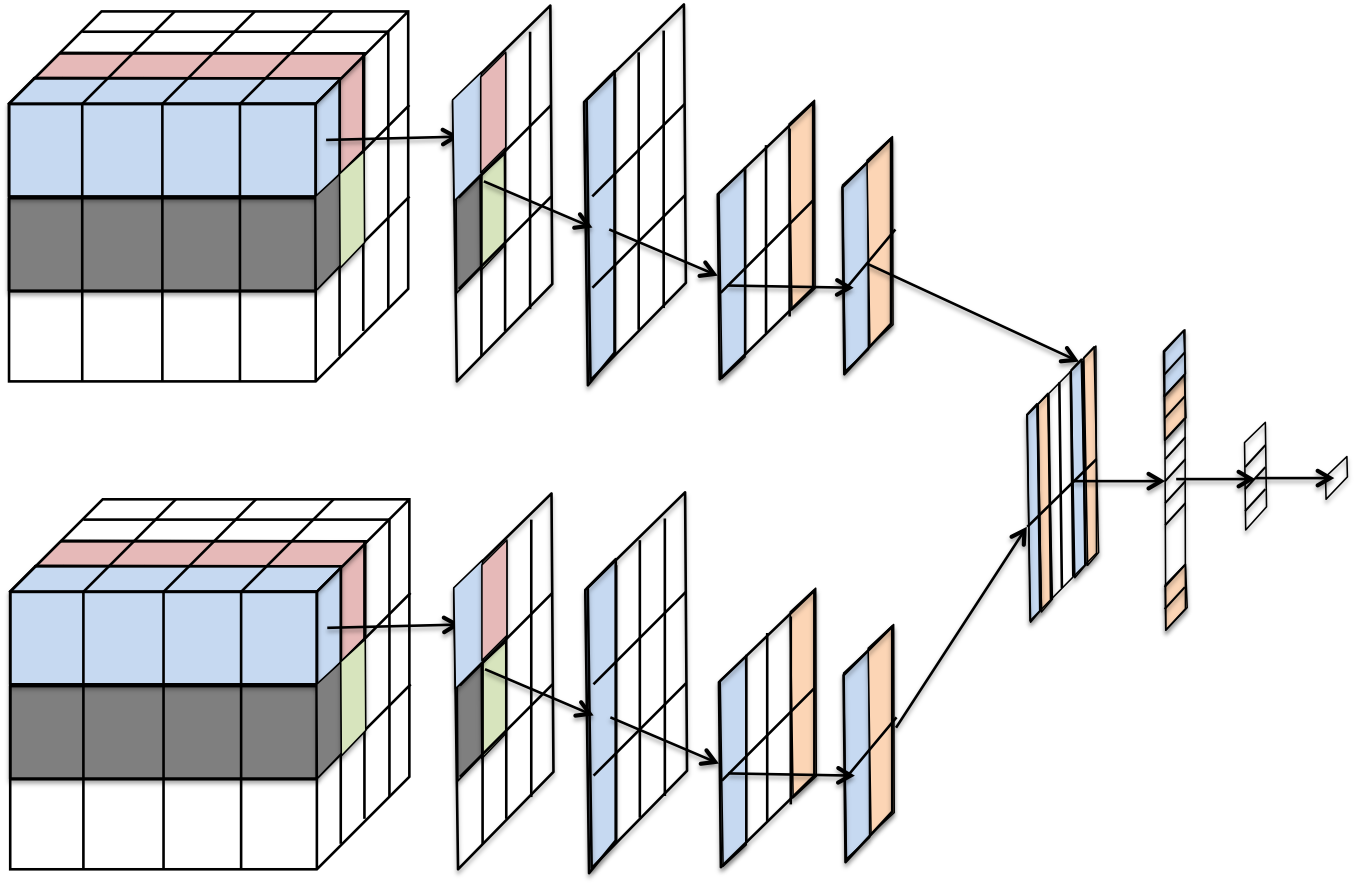
\includegraphics[width=85mm]{pictures/Conceptual}
    \caption {A synthetic image classification pipeline with elements mapping highlighted in color scheme. 
    \textcircled{1}: Conversion of multi-channel image to gray scale.
    \textcircled{2}: Local feature extraction.
    \textcircled{3}: Vector dimension reduction.
    \textcircled{4}: Vector sampling.
    \textcircled{5}: Conversion from float to double.
    \textcircled{6}: Vector combining.
    \textcircled{7}: Matrix vectorizing.
    \textcircled{8}: Lineage model prediction.
    \textcircled{9}: Selection of the index with maximum value.
    \label{fig:conceptual}
}
\end{center}
\end{figure}

The performance penalty introduced by lineage capturing comes mostly from persisting in-memory data to storage.
In the context of data transformation, there are three potential datasets: the input, the output, and mapping between them.
Recording only the metadata (coordinates) mapping rather than the actual data value places a lower bound of the amount
of data the lineage system needs to capture. The actual dataset can be derived by rerunning the pipeline.
Among the mapping types, geometry mapping takes more storage space than others due to the arbitrary between two collections
of metadata. We introduce an high-order function approach to describe each geometry and record the mapping between
each pair of geometries to reduce the storage consumption. We also investigate various indexing strategies for better
query performance for geometry mapping.

We present Gineala, a lineage collecting and serving system that implements the above general solutions.
Gineala is integrated with the KeystoneML~\cite{sparks15} distributed machine learning framework.
KeystoneML exposes two building blocks: transformers and estimators. 
A transformer applies a deterministic unary function to data items and produce new data items.
An estimator takes a collection of data items, and feed them to a training procedure,  and produces a transformer.
Gineala interacts with KeystoneML at the Transformer level, where the users can declare the lineage type and instrumentation.
Gineala collects five types of data for each Transformer: the input dataset, the output dataset, the mapping between them
along with the computation and the optional model.
Gineala stores the lineage information on HDFS~\cite{shvachko10} via the resilient distributed dataset (RDD) abstraction
of Apache Spark~\cite{zaharia12}, the underlying computing engine of KeystoneML.
Upon query, Gineala can load the lineage information from storage and reconstruct the lineage chain.
Users have the flexibility to specify either to reconstruct a single transformer lineage, a partial chain, or the whole chain.

By examining the KeystoneML code base, we see that Gineala's lineage interface covers 87\% (39 out of 45) of the existing transformers.
Combining the high-order function approach and spatial indexing strategies, 
the geometry lineage query runs 2x-31x \evannote{do you just want so say ``up to 31x'' in the intro} faster and storage consumption is reduced from $O(kN^2)$
to $O(k)$, assuming k is the number of mappings, N is the number of input and output elements in each geometry. 
Our measurements with the three representative ML pipelines show that Gineala lineage capturing scales no worse than the
ML pipelines.
The performance penalty for the three fore-mentioned use cases ranges from 16\% to 54\%.
The query for these use cases takes from 0.1~s to 1.8~s. \evannote{Is this low enough that you can claim interactive response times on lineage queries?}

In summary, we make the following contributions:
\begin{shortlist}
\item{} We present a concise and powerful lineage system interface by formulating the cell-wise mapping in ML pipelines as multi-dimensional space transformation.
\item{} We present a high-order function to describe the geometry to reduce storage overhead.
\item{} We present and evaluate various spatial indexing strategy to improve the query performance.
\item{} We present the lower and upper bound of the amount of data that needs to be collected to enable complete pipeline lineage.
\item{} We present three real uses case of using fine-grained data lineage for data, code, and results debugging, respectively.
\end{shortlist}

%The rest of the paper is organized as following: 
%\S\ref{sec:Background} introduces the background of KeystoneML and typical uses of fine-grained lineage systems. 
%\S\ref{sec:Lin} discusses lineage of a machine learning pipeline formally.
%\S\ref{sec:Design} discusses the general design of Gineala.
%\S\ref{sec:Impl} documents the Gineala implementation on KeystoneML with technical details
%We present the performance measurements in \S\ref{sec:Perf}.
%\S\ref{sec:Related} surveys existing lineage systems.
%We conclude and envision future work in \S\ref{sec:Conclusion}.

\section{Background}
\label{sec:Background}
In this section, we briefly review the KeystoneML and introduces three use cases of Gineala.

\subsection{KeystoneML}
KeystoneML is an application framework designed for the implementation of robust large-scale machine learning pipelines. Built on the principles of declarative programming and modular design, KeystoneML provides a light-weight and elegant API that allows users to describe these pipelines as the composition of two types of operator--Transformers, which perform deterministic data transformation, and Estimators, which ``learn'' Transformers based on training data. KeystoneML pipelines are fit and executed in parallel using Apache Spark. These pipelines are compiled into an application DAG and optimized before execution. Current optimizations include online decisions about materialization of intermediate state, as well as standard optimizations such as common subexpression elimination. KeystoneML includes a library of standard feature extractors in domains including computer vision, audio, and text processing, as well as standard statistical procedures and Estimators for several types of machine learning model.

\subsection{Use Cases}
We select three use cases from real ML pipelines, these three cases are representative for data debugging, code debugging, and results debugging, respectively.

\subsubsection{Data Debugging}
Figure~\ref{fig:mnistrandomfft} shows the MNISTRandomFFT pipeline that classifies hand written digits. 
The user of this pipeline trains the linear model by feeding the prepared datasets (results of VectorCombiner) to the Linear Solver.
After deploying the trained model, the user finds a corrupted data item in the training dataset and he wants to replace the erroneous model
with the correct model. 
As a straightforward solution, he can clean the dataset by removing the corrupted data item and rerun the whole pipeline.

While the fine-grained data lineage information provides an opportunity to avoid repeating the whole pipeline.
Specifically for this use case, we chain the lineage information from the beginning of the pipeline till VectorCombiner.
With forward query and backward query, we confirm that the corrupted data item, a 784 dimensional vector, only affects
a 2048 dimensional vector as the output of VectorCombiner, and vice versa. So instead of rerunning the whole pipeline, 
we can filter the output of VectorCombiner to remove the corresponding vector, and feed the filtered dataset to the linear solver.
In this way, debugging latency is reduced by skipping the repeated computation in the pipeline.

\begin{figure}[ht]
\begin{center}
    \includegraphics[width=85mm]{pictures/MNISTRandomFFT}
    \caption {The MNISTRandomFFT pipeline, boxes are dataset, rounded-corner boxes are transformers, dashed rounded-corner boxes are estimators.
    \label{fig:mnistrandomfft}
}
\end{center}
\end{figure}

\subsubsection{Code Debugging}
Another use of pipeline lineage information goes beyond understanding a single pipeline in isolation.
In this use case we use lineage as a tool in the debugging process as pipelines change and are augmented. 
Typical machine learning workflows are constructed via an iterative proces of refinement with a machine learning developer or data scientist in the loop.
These users are constantly engineering new features, adding new datasources, and trying out new machine learning methods at all stages of the pipeline.
Lineage offers a natural way for these users to hone in on the areas where two similar pipelines diverge in terms of their intermediate data, and presents a new avenue for investigation of model performance by allowing users to pinpoint the point at which their data diverged from a known good pipeline and to inspect \emph{what} changed during the data processing procedure. 


\begin{figure}[ht]
\begin{center}
    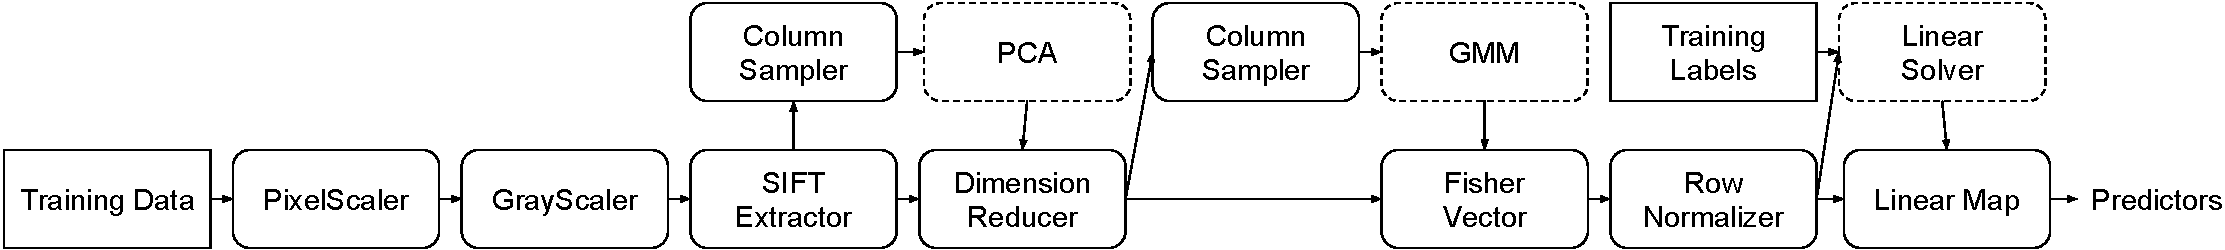
\includegraphics[width=85mm]{pictures/VOCSIFTFisher}
    \caption {The SIFTFisher pipeline, boxes are dataset, rounded-corner boxes are transformers, dashed rounded-corner boxes are estimators, shaded boxes are calling out to C library for computation.
    \label{fig:vocsiftfisher}
}
\end{center}
\end{figure}

As a concrete example, consider the SIFTFisher pipeline, shown as Figure~\ref{fig:vocsiftfisher}. 
It has been shown that augmenting traditional SIFT (Scale-invariant feature transform) descriptors with additional location information about the location of the descriptor in the input image can improve classification performance.
However, when we first developed such a pipeline, our results conflicted with published work indicating that these features provided a statistically significant improvement in classification accuracy.
By employing lineage based debugging, we could isolate exactly where in the pipeline our calculations diverged from the original features, and diagnose impacts seen downstream like a under-fit GMM (Gaussian Mixture Model), and trace the ultimate lack of classification improvement to a bug in the underlying C library which we called into.
By visualizing the features we could see that the new features added to our model did not correspond to positions in the image, but rather contained values outside of a suitable range for these features, which turned out to be randomly allocated memory. The SIFT feature visualization involves backward query on the lineage of the SIFTExtractor transformer and highlights of the corresponding input pixels.


\subsubsection{Results Debugging}
Users of ML pipelines often interpret the results, identify some potential data anomalies, then retrospect the supporting input data for better understanding.
Fine-grained data lineage of ML pipelines have sufficient information for such investigation.

\begin{figure}[h]
\begin{center}
    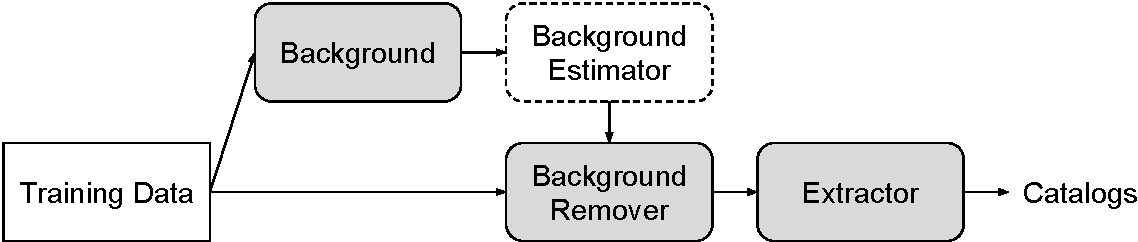
\includegraphics[width=85mm]{pictures/SourceExtractor}
    \caption {The SourceExtractor pipeline, boxes are dataset, rounded-corner boxes are transformers, dashed rounded-corner boxes are estimators, shaded boxes are calling out to C library for computation.
    \label{fig:sourceextractor}
}
\end{center}
\end{figure}

One such use case is results validation in the SourceExtractor pipeline, shown in Figure~\ref{fig:sourceextractor},
that processes images from the telescopes and produces astronomical object catalogs. 
The astronomical object catalog includes the position, shape, and other statistical properties of the object.
In this case, astronomers find the bright objects over a threshold and validate that these objects are indeed astronomical objects rather
than noise caused by cosmic rays.
With the lineage information, astronomers can first filter the results to find the objects whose brightness is above a threshold.
Then using backward query, they can find corresponding pixels for these bright objects. 
Either through mathematical analysis or human intervention, they are able to validate the correctness of the bright objects.

\section{Lineage}
\label{sec:Lin}
In this section, we formally define the notion of pipeline, dataset, lineage and its associated operations of query and replay.

\subsection{Pipeline and Datasets}
\label{sec:Lin-Pipe-Data}
We define a dataset $I$ as a collection of structured data. In the scope of this work, the supported structures are: 
string, vector, matrix, and image. A vector or a string is a one dimensional data structure and a matrix is two dimensional. 
For simplicity, we view string as a vector.
An image is a three dimensional data structure that is defined by the height, the width and the number
of channels. Putting these data structures in a collection, e.g. a RDD or a sequence, introduces one additional dimension.

An element $e \in I$ has two properties: value $e.value$ and coordinates $e.coor$. 
Combining the additional dimension in the collection with the data structure, 
the coordinates of an element is a pair of integers, a triple of integers, or a quadruple of integers
for vector, matrix, and image, respectively.

A pipeline $P$ is defined as a sequence of transformers $(T_1, T_2, ..., T_n)$. 
Each transformer $T_i$ takes a dataset $I_i$ as its input, and produces $I_{(i+1)}$ as the output. 
Especially, we denote the output of the whole pipeline as $O = I_{n+1}$

\subsection{Dataset Companion}
Since transformers operate at the data structure (DenseVector, DenseMatrix, Image) level, we use the notation
$\overline{I_i(e)}$ as the companion of $I_i$ with respect to element $e$ such that $\forall a \in \overline{I_i(e)}$,
\[ a.value =
  \begin{cases}
    e.value       & \quad \text{if } a.coor = e.coor\\
    NaN  & \quad \text{otherwise}. \\
  \end{cases}
\]

Accordingly, given a list of distinct elements $(e_1, ..., e_m)$, the companion of $I_i$ with respect to $(e_1, ..., e_m)$ is
described as: $\forall a \in \overline{I_i(e_1, ..., e_m)}$, 
\[ a.value =
  \begin{cases}
    e.value       & \quad \text{if } \exists e \in (e_1,...,e_m), a.coor = e.coor\\
    NaN  & \quad \text{otherwise}. \\
  \end{cases}
\]


\subsection{Data Lineage and Replay}
Before defining the lineage, we need to introduce the relationship between the two data structures $A$ and $B$ with the same type.
We say $A \subseteq B \text{ or } B \supseteq A$, $\text{if }\forall a \in A, \exists b \in B, s.t.\text{ } a \neq NaN \land a.coor = b.coor \land a.value = b.value$.
By saying $A = B$, we mean $A \subseteq B \land B \subseteq A$.

We define the data lineage of a given element as the elements in the input dataset that is used to produce present element.
The single transformer lineage is
\begin{equation}
S(e \in I_{i+1}) = \{e_1, ..., e_m | T_i(\overline{I_i(e_1, ..., e_m)}) \supseteq \overline{I_{i+1}(e)}\}.
\label{equa:SingleLineage}
\end{equation}


Recursively, the lineage of a given element across multiple transformers can be defined as
\begin{equation}
L(e) = \cup_{e' \in S(e)} L(e').
\end{equation}

We define the property of $Replay(e \in I_{i+1}) = \overline{I_{i+1}(e)} \subseteq T_i(\overline{I_i(e_1, ..., e_m)})$ in Equation~\ref{equa:SingleLineage}
as the replay property, which means we can reproduce the output solely with its lineage and the corresponding transformer.
The constraint of the replay property is that only the element $e$ is guaranteed to be the same as the original transformation 1
if $\overline{I_{i+1}(e)} \subseteq T_i(\overline{I_i(e_1, ..., e_m)})$. In this case, the results of the replayed transformer may
produce inconsistent results for elements other than $e$ in $I_{i+1}$. 
In some cases, we see a stronger condition of $\overline{I_{i+1}(e)} = T_i(\overline{I_i(e_1, ..., e_m)})$, which indicates that
the replayed results are exactly the same as the original results.

The replay property for multiple elements require the lineage for all elements. Formally,
$Replay(e_1,..,e_m \in I_{i+1}) = \overline{I_{i+1}(e_1,...,e_m)} \subseteq \cup_{e \in (e_1,...,e_m)} Replay(e) $.

\subsection{Data Lineage Query}
The forward query of an element over data lineage of a pipeline $P$ returns $qForward(e) = \{e' | e \in L(e' \in O)\}$. 
And the backward query of an element over data lineage returns $qBackward(e) = e' \in L(e)$.
Specifically, the identifier of an element is its coordinates in the according data structure, so the query actually takes
the coordinates of the input element as key, and query over the data lineage. The query that spans multiple transformers 
use coordinates as intermediate data. Once the query reaches the final transformer, it associates the actual values
with the result element coordinates and return them.

Queries of multiple elements can then be expressed as the union of the query for each element: 
\begin{equation}
\begin{split}
qForward(e_1, ..., e_m) = \cup_{e \in (e_1, ..., e_m)} qForward(e) \\
qBackward(e_1, ..., e_m) = \cup_{e \in (e_1, ..., e_m)} qBackward(e).
\end{split}
\end{equation}

\section{Requirements}
\label{sec:Req}
The requirements of the Gineala lineage system for KeystoneML can be viewed from the functionality and performance perspective.

\subsection{Functional Requirements}
Gineala should expose a programming interface for users to declare and operate the lineage of each transformer. 
Gineala's built-in lineage should cover the most common lineage types and preserve the flexibility for users to declare their own lineage types.
Gineala also requires an interactive interface for users to load recorded lineage and query over it.

The single transformer lineage need to provide the forward query and backward query functionalities. 
It is  guaranteed that the lineage across transformers can be queried in a chain, as long as the transformers
can form a pipeline (the transformers' types conform the pipeline strong type checking).

The single transformer lineage should be able to be replayed deterministically, meaning that with the same input dataset and transformer,
the lineage can reproduce the identical result and the original result even with the presence of random factors.
In turn, a partial pipeline assembled by a sequence of transformers of the original pipeline should be able to be replayed deterministically.

\subsection{Performance Requirements}
\label{sec:Req-Perf}
As Gineala incurs additional computation and I/O to record and save lineage, the overall pipeline performance is expected to slowdown.
Especially for KeystoneML that is built upon Apache Spark, unlike other distributed computing framework such as Hadoop~\cite{HADOOP} 
that writes/reads intermediate data to disk, any additional I/O can introduce a more significant slowdown. 
The Hadoop-based lineage system Newt~\cite{logothetis13} reported a 20$\sim$50\% slowdown; 
another Hadoop-based lineage system GMRW~\cite{ikeda11} observed a slowdown of 16$\sim$76\% depending on the workloads;
the SciDB~\cite{brown10}-based SubZero~\cite{wu13} system introduced 50$\sim$150\% overhead. 
We expect Gineala's slowdown to the original pipeline to be comparable to these systems.

When Gineala records lineage, we face tradeoffs between performance slowdown, memory usage and disk space.
In some cases, it may run additional computations on the collected lineage to reduce the lineage size. 
E.g., regressing a sequence of coordinates to a higher order function. 
In other cases, it may cache all lineage information for a transformer before writing it to the storage. 
Gineala should be able to automatically instrument the lineage collection to adapt the constraints.

Lineage information can be massive depending on the transformer, since the input dataset or the intermediate dataset of a pipeline can be large.
In some transformers, the mapping between the input elements and output elements is complicated. 
Regress the element-wise mapping to a higher order function can reduce the storage overhead, however it introduce latency when users
query them. Thus Gineala requires indexing strategies for the recorded lineage to overcome this issue.

\section{Design}
\label{sec:Design}
Figure~\ref{fig:architecture} shows the overview of Gineala and its interactions with other components. 
Rounded-corner rectangles are components around and inside KeystoneML. 
The two-sided arrows indicate interactions between components.
Users compose machine learning pipelines with KeystoneML and submit the compiled DAG to Spark.
All computation and I/O are done through the Spark Resilient Distributed Dataset (RDD) abstraction.
With Gineala, users can declare and operate lineage at the transformer level, 
so that the compiled DAG also contains lineage recording and other operations, e.g., save to disk.
Lineage in Gineala is stored to HDFS~\cite{shvachko10} via Spark's RDD abstraction.
Users can load the stored lineage in HDFS to Spark interactive command line interface.
By calling Gineala primitives, users can query elements of interest, replay transformers, or analyze
the lineage for other purposes.

\begin{figure}[h]
\begin{center}
    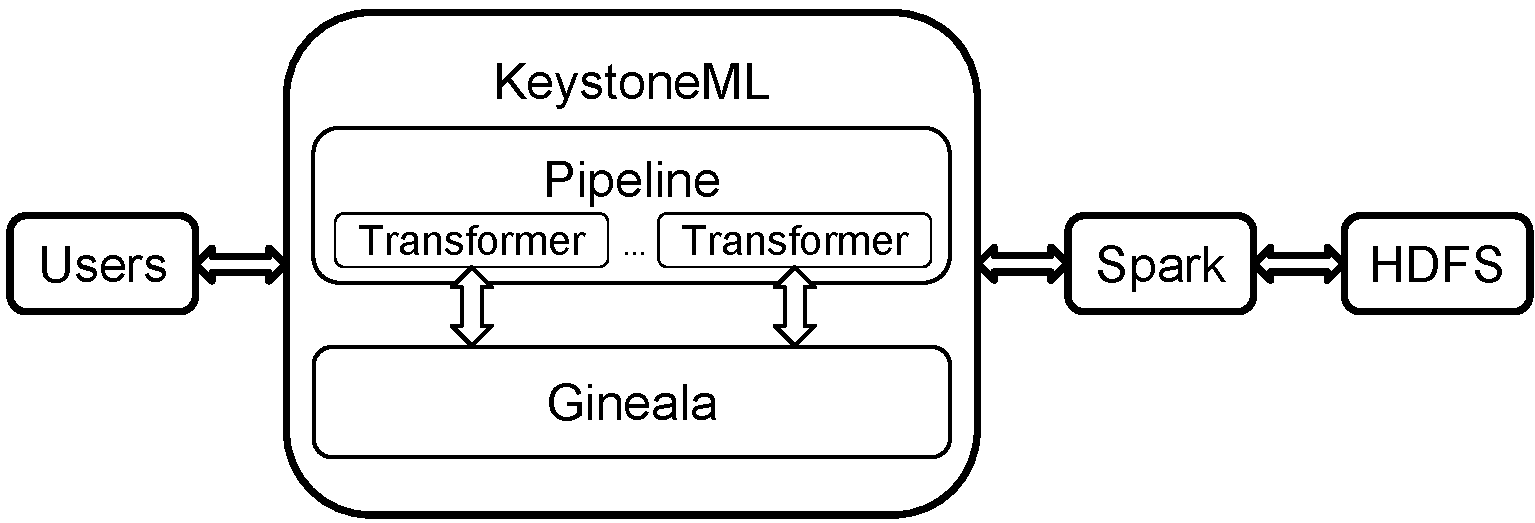
\includegraphics[width=85mm]{pictures/architecture}
\caption {Overview of Gineala and its surrounding components.
    \label{fig:architecture}
}
\end{center}
\end{figure}

\subsection{Lineage}
\label{sec:Design-Lineage}
For each transformer, Gineala collects five types of data: the input dataset, the output dataset, the transformer, the collection of mapping, the model, and the random parameter.
The model stores the trained model of an estimator generated transformer.
The random parameter holds the information that guarantees the determinism of the transformer.

For estimators, we only consider linear model estimators in the current implementation. 
We view linear model estimators as transformers without model or random parameters, 
but instead we keep track of the training parameters that are used to obtain the output model (the output dataset). 

\subsection{Mapping}
\label{sec:Design-Mapping}
Mapping is a notion that describes the element-wise dependency in Gineala. 
It is an abstraction that is independent from specific data structure in the scope of DenseVector, DenseMatrix, and Image.

Consider a transformer that transforms a RDD of matrices to another RDD of matrices.
A RDD of matrices can be understood as a distributed array of matrices that is distributed across a cluster.
We observe that many transformations in various pipelines has narrow dependencies, where a output matrix
only depends on one input matrix. Figure~\ref{fig:narrowmapping} shows this case. 
The left mapping is from an input RDD of matrices to an output RDD of matrices. 

\begin{figure}[h]
\begin{center}
    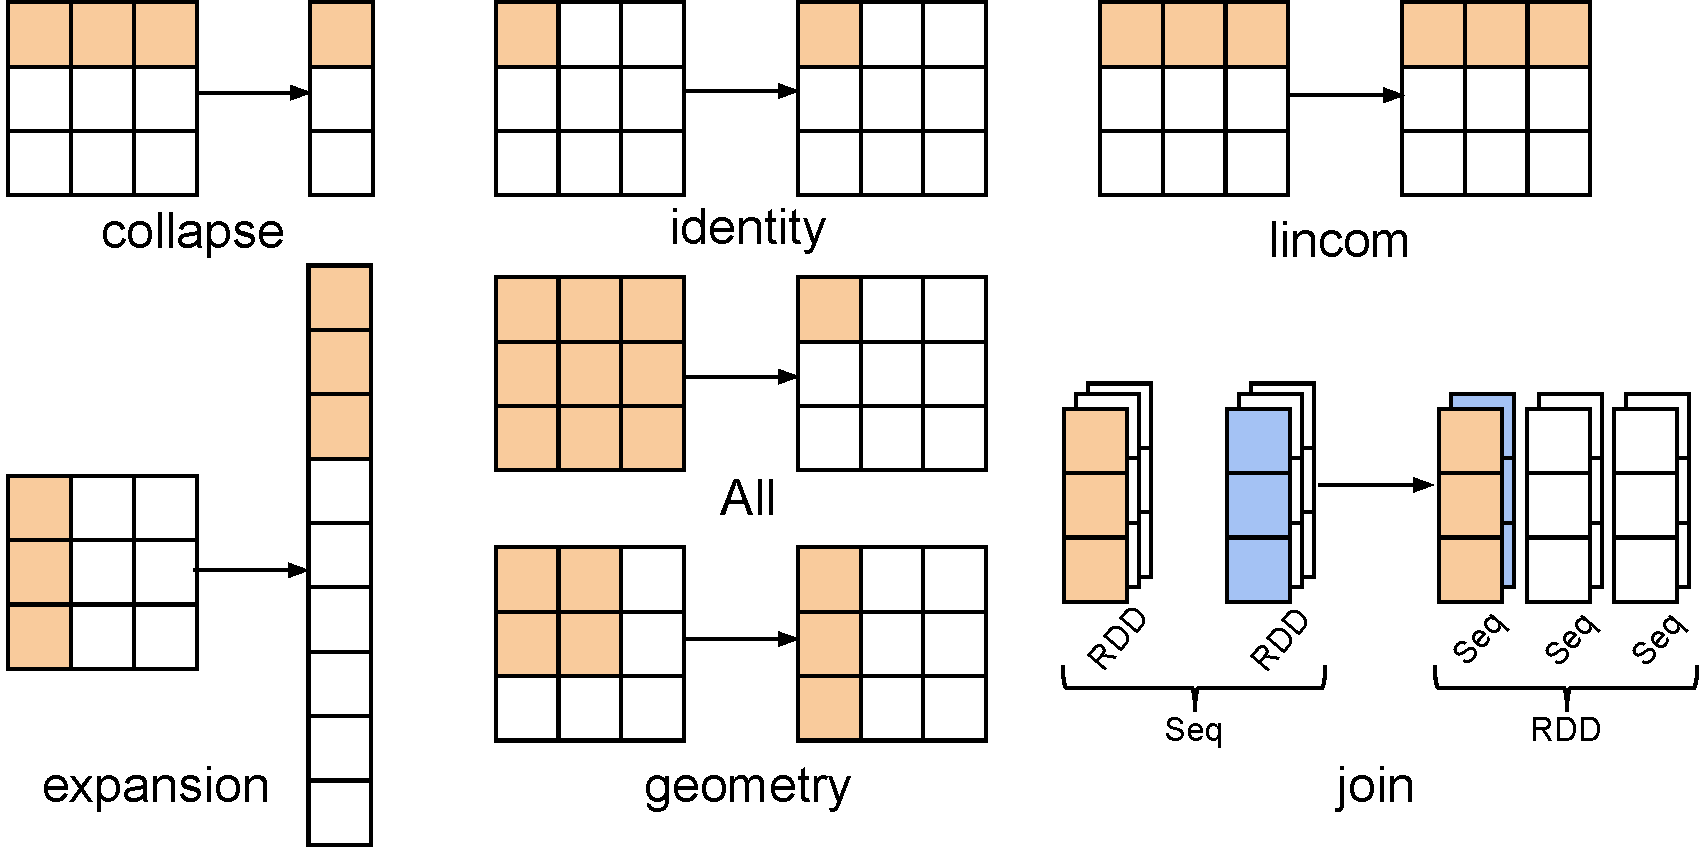
\includegraphics[width=85mm]{pictures/narrowmapping}
\caption {Left: The narrow mapping cases in the context of Resilient Distributed Dataset (RDD), rectangles are RDDS and rounded-corner rectangles are matrices.
Right: Four element-wise mapping cases, mappings are shown with color highlights.
    \label{fig:narrowmapping}
}
\end{center}
\end{figure}

Taking a pair of matrices, we see four types of element-wise mappings: 
{\bf One Mapping}, in which case each output element only depends on one element with the same coordinate in the input matrix.
{\bf All Mapping}, in which case each output element depends on all elements in the input matrix.
{\bf Region Mapping}, in which a group of output elements depend on a group of input elements.
{\bf Sample Mapping}, in which the output is a sample of the input.

In general, all three data structures, DenseVector, DenseMatrix and Image have these four mapping types. 
So Gineala defines these four element-wise mapping types, and users can use these mapping types to declare lineage. 
In the next section, we will introduce how Gineala's lineage interface exposes the lineage declaration interface with the mapping information.


\subsection{Region Mapping}
\label{sec:Design-RegionMapping}
As can be seen in the region mapping example in Figure~\ref{fig:narrowmapping}, the backward query of an output element should return all the input elements in the corresponding region. If the output region has $N$ elements and the input region has $N$ elements, the space complexity of storing such a mapping is $O(N^2)$. 
Inspired by the Scale-invariant feature transform (SIFT) and the SourceExtractor implementation, each of them processes an input matrix and produces thousands of vectors as outputs. An output vector depends on a group of elements in the matrix, and these elements form a two dimensional shape. 
For SIFT, the input elements form a circle with a geographical center and the scale as its radius.
Similarly, the SourceExtractor's input elements  form an ellipse. 
Gineala uses a higher-order function to describe the region. 
Thus the mapping between two regions is expressed as a tuple of two higher-order functions.
The space complexity goes down to O(1).

Since many softwares such as SIFT and SEP already return the geographical information with the results.
Gineala exposes some simple interfaces for two dimensional shapes as special cases.
Users can pass in the geographical information directly to declare rectangle, circle, and ellipse.

Using the higher order function involves an issue for query. If the mapping is recorded at the element level, query is straight forward.
Given an output element, a backward query returns corresponding input elements.
Now both the input elements and output elements are encoded with a higher order function. 
And the mapping between input function and output function is stored in a list. 
A query that takes an output element as key thus needs to iterate over all input functions and test if the key is in the function or not.
If the key is in an input function, it then returns the mapping output function, and expands the function to a group of coordinates.
The time complexity of query over Region Mapping is then $O(N^2)$, assuming there are $N$ tuples in the list and each input function expands to $N$ elements.
To speedup the query performance, we implement and compare several indexing strategies, and a detailed discussion is in \S\ref{sec:RegionIndex}.

\subsection{Lineage Type}
Gineala defines three lineage interfaces at high level: NarrowLineage, GatherLineage, LinComLineage. 
NarrowLineage covers the lineage that has a narrow dependency and GatherLineage covers the dependency in a gather pattern, where the transformer takes a sequence of RDD of data structures and transform them into a single RDD of data structures. 
LinComLineage is for the transformer which is the output of fitting training dataset to the linear model estimator.

The NarrowLineage can then be further specified with a specific mapping pattern. E.g., NarrowLineage that has One Mapping is named as OneLineage.
For OneLineage and AllLineage, the users only need to pass the input dataset, output dataset, and the parameters, since Gineala can figure out the element-wise mapping from the metadata of the internal data structure.

For RegionLineage and SampleLineage, Gineala requires the mapping collection for the declaration. 
Such a collection should be a RDD of tuple list. 
Each tuple is a pair of the input region and the output region.

The GatherLineage is implemented within the GatherTransformer.
And so is LinComLineage for the linear model estimator. LinComLineage requires the model as input for declaration.
Both these two lineage types can adapt to DenseVectors, DenseMatrix, and Images. 
Users do not have to modify these two lineage types. 

\section{Implementations}
\label{sec:Impl}
This section discusses implementation details for lineage collection, I/O, and region mapping index.

\subsection{Metadata Separation}
As discussed in \S\ref{sec:Req-Perf}, writing lineage to persistent storage can introduce a more dramatical slowdown for KeystoneML comparing
to the Hadoop-based systems, since Spark seeks to eliminate unnecessary I/O between memory and persistent storage.
One effective way to reduce the I/O overhead is reduce the lineage data size.

Gineala reduces the lineage data size by 1) separating the metadata from the datasets, 2) tracking only the metadata mapping, 
and 3) taking advantage of the mapping types specified by the user.

In \S\ref{sec:Lin-Pipe-Data}, we say an element in a data structure has two properties: the coordinate and the value.
We refer the coordinate as the metadata of a particular element and the value as the actual data. 
In a backward query of an element throughout the whole pipeline, the query traverses from the last transformer
to the very first transformer in a sequential manner. 
We see that in the last the transformer and other transformers in the middle, the metadata mapping is sufficient to answer
the query of depending input elements of given output elements. Only in the very first transformer do we need both the metadata
to find the metadata of the depending input elements and the actual data of these elements.
So Gineala separates the metadata from actual data and only tracks the metadata mapping.

Another lineage size reduction is contributed by user specified mapping types. 
The {\bf One Mapping} and {\bf All Mapping} are the mapping types behind the OneLineage and AllLineage, respectively.
Both the two mapping types are symmetric.
In {\bf One Mapping} if an output element depends exactly on the input element with the same coordinate, 
the input element value only propagates to that only output element. 
Thus both the forward and backward query return the element that has the identical coordinate as the key.
So is for {\bf All Mapping}, the dependency of all input elements to an output element indicates that every input element's value propagates to all output elements.
Both the forward and backward query shall return all elements in the data structure.
Thus for {\bf One Mapping} and {\bf All Mapping}, recording the metadata of the matrix is enough to answer the forward and backward query.

In contrast, the {\bf Region Mapping} and {\bf Sample Mapping} are asymmetric. 
{\bf Sample Mapping} is implemented as a subtype of {\bf Region Mapping}, as it samples a random subset of the input data structure and return that subset as output.
We can describe the subset as a list of random regions (rectangles in column sampling of a matrix), with each input region maps to an output region.
To record these two mapping types, metadata of data structures is not sufficient to answer the queries. 
Gineala needs to record region level mappings instead.

Putting all lineage size reduction strategies together, 
a profile study of the VOCSIFTFisher pipeline shows that the actual data size is 840.9~GB and the metadata size is 61.3~GB. 
Writing only metadata can reduce the total I/O amount by a factor of 13.7x.

For the actual data, Gineala only stores the input dataset for the very beginning transformer as mandatory. 
Users can configure the Gineala to make decisions for other transformers' input and output datasets.




\subsection{Actual Dataset Storage}
In the previous section, we introduce how Gineala separates the metadata from actual data and saves the metadata mapping.
However, Gineala still needs the actual data to answer the forward and backward query.

Considering a multi transformer pipeline, with each transformer having its own input dataset and output dataset.
The minimal actual dataset Gineala needs to save to persistent storage is the input dataset for the very beginning transformer, as
the rest datasets can be reproduced by rerunning the pipeline with the input dataset.

Intuitively, the maximal actual dataset Gineala can save to persistent storage contains all input datasets and output dataset for each transformer.
Since a transformer's output dataset is also the input dataset for the succeeding transformer, thus the maximal dataset without duplicates
should include output datasets of all transformers and the input dataset for the beginning transformer. 

Fundamentally, this is a tradeoff between pipeline slowdown, storage space consumption and query overhead. 
Storing the minimal actual dataset consumes the least space on disk along with the least writing overhead, 
but access to the actual dataset other than the input introduces overhead due to reexecution of the pipeline or a part of the pipeline.
Storing the maximal dataset consumes more disk space and more time, but queries over the actual dataset
have a lower latency.

Assuming Gineala collects lineage information that is complete for the whole pipeline, the space formed by the storage overhead 
(slowdown depends on the storage overhead) and query overhead defines users' flexibility to make actual dataset storing decision.

In other cases, users are only interested in one or few transformers. E.g. debugging the transformer implementation.
He may preempt that transformer's lineage by recording all its input and output dataset. 
And no lineage from other transformers is needed.
Gineala supports such flexibility by letting the user declare and operate lineage for one or few transformers.
In turn, the lineage collected in this case only supports query over each individual transformer.
It these transformers form a sub-pipeline, users can query the lineage throughout this sub-pipeline with Gineala.

As introduced in \S\ref{sec:Design-Lineage}, Gineala collects six types of data for lineage: the input dataset, the output dataset,
the transformer itself, the mapping collection, the model, and the parameter.
Among these six data types, the transformer and the collection of mapping are mandatory. 
The input dataset is mandatory if the transformer is the very first of the pipeline. 
Otherwise, the input dataset is optional.
The output dataset is optional, as it can be reproduced by rerunning the transformer with the input dataset.
The model and parameter are optional.

In terms of data size, the input dataset, the output dataset and the mapping collection is dominant. 
Since all of these three datasets are of the type of RDD abstraction, Gineala calls the RDD primitive to write these datasets
to HDFS, so that each partition is written into the local disk. 
And loading these RDDs from HDFS can benefit from the locality.
For other data types, we encapsulate them into a RDD and use the same approach to write them to HDFS.

All these six datasets are written into a directory that is named by concatenating the transformer label, 
the node sequence id in the pipeline, and the id of the initial input dataset. 
With id of the initial input dataset, Gineala can figure out the branches of the pipeline.
By looking into the input/output RDD id, Gineala is able to tell the sequence of each transformer in the pipeline.
Combining the two previous operations, Gineala can build the lineage of a pipeline in the exact same sequence
as the original pipeline.

\subsection{Region Mapping Index}
\label{sec:RegionIndex}
In \S\ref{sec:Design-RegionMapping}, we introduced the notion of region mapping and how we user higher-order function
to describe the region for the purpose of less space consumption. We also present that query of such region mapping
can be slow due to the encoding. 
In this section, we discuss four indexing strategies to speedup the query over the region mapping. 
The four indexing strategies are referred as {\bf NoIndex}, {\bf Direct}, {\bf RTree}, and {\bf KMeans}, respectively.
For simplicity, we only discuss forward query from the input to the output in this section.
The backward query works in the same way as the forward query.


We use the example in Figure~\ref{fig:example} in the following discussion.
\begin{figure}[h]
\begin{center}
    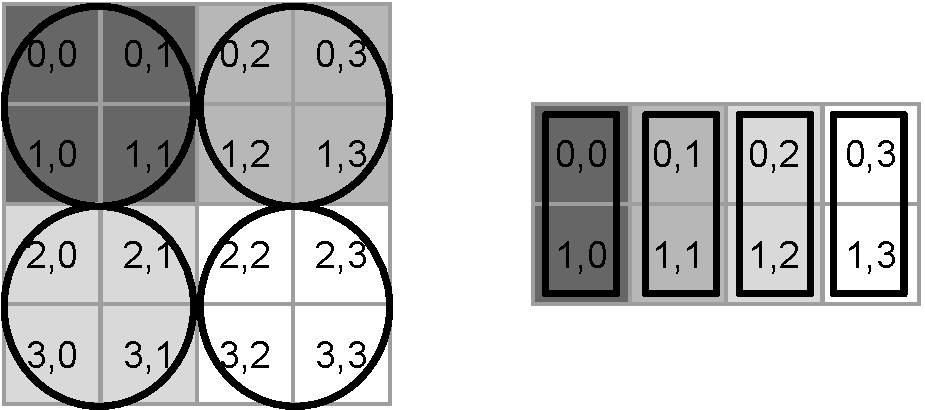
\includegraphics[width=85mm]{pictures/example}
\caption {A region mapping example, the left matrix is input and the right matrix is output. The mapping between the regions are shown using gray shades.
    \label{fig:example}
}
\end{center}
\end{figure}

Table~\ref{tb:example} shows the mapping for each element and the regressed 2D region mapping.
\begin{table}[ht]
\begin{center}
    \caption{Element-wise mapping and regressed region mapping of the example in Figure~\ref{fig:example}}
    \begin{scriptsize}
    \begin{tabular}{ | p{1.75cm} | p{1.75cm} | p{1.75cm} | p{1.75cm} |}
    \hline
    Input & Region & Output & Region \\ \hline \hline
    (0,0),...,(1,1) & Circle\_0 & (0,0),(1,0) & Rect\_0 \\ \hline
    (0,2),...,(1,3) & Circle\_1 & (0,1),(1,1) & Rect\_1 \\ \hline
    (2,0),...,(3,1) & Circle\_2 & (0,2),(1,2) & Rect\_2 \\ \hline
    (2,2),...,(3,3) & Circle\_3 & (0,3),(1,3) & Rect\_3 \\ \hline
    \end{tabular}
    \end{scriptsize}
    \label{tb:example}
\end{center}   
\end{table} 

\subsubsection{No Index}
Using the example in Table~\ref{tb:example}, with {\bf NoIndex} strategy, query an element needs to traverse all circles (input regions).
If the element is in a circle, the query returns the all output elements expanded from the mapping rectangle.
The time complexity of a query is $O(N)$, where N is the number of circles. 

\subsubsection{Direct Index}
To build the {\bf Direct} index, we use each input element as key and the associated region as the value, as shown in Figure~\ref{fig:direct}.
We rely on the underlying runtime system for the optimization of storing repeated regions as an single object,
then use an pointer (hash value of the object) to point to the region object, as shown in Figure~\ref{fig:direct-optimized}.
This optimization can reduce the storage space of index if the region object is larger than the hash value. 
A query of an element takes two steps: the first step returns the hash value for that element and the second step returns the rectangle. 
The space complexity of {\bf Direct} index is $O(k*N)$, where $k$ is the number of circles and $N$ is the number of elements in each circle.
For simplicity, the space complexity of the {\bf Direct} index is $O(N^2)$.
The time complexity of building index and query are $O(N^2)$ and $O(1)$, respectively.

\begin{figure}
\centering
\begin{minipage}{.3\linewidth}
  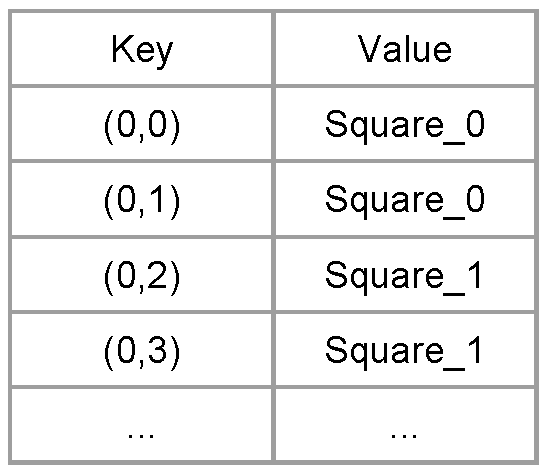
\includegraphics[width=\linewidth]{pictures/direct}
  \caption{Direct index}
  \label{fig:direct}
\end{minipage}
\hspace{.05\linewidth}
\begin{minipage}{.6\linewidth}
  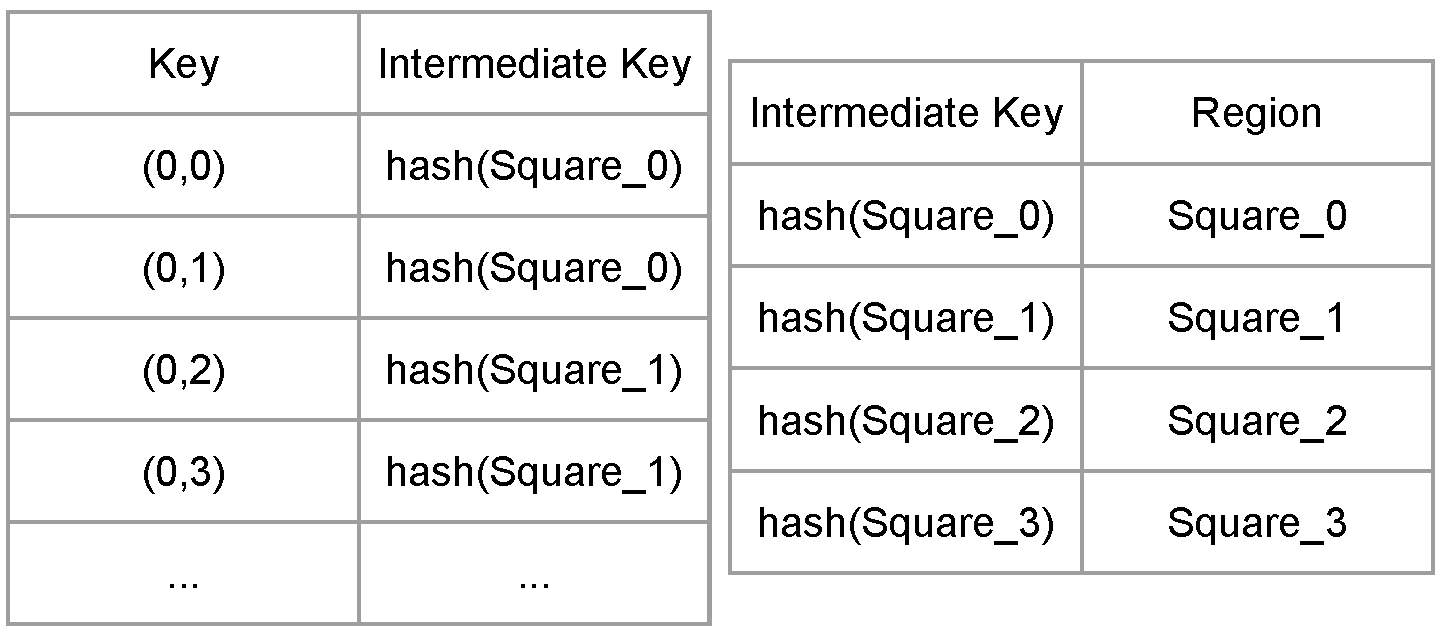
\includegraphics[width=\linewidth]{pictures/direct-optimized}
  \caption{Direct index with optimization}
  \label{fig:direct-optimized}
\end{minipage}
\end{figure}


\subsubsection{RTree Index}
R-tree~\cite{guttman1984} has been introduced to index multidimensional information.
To simplify the discussion, we use the example shown in Figure~\ref{fig:example} and build the index in a two dimensional space.
The average query time complexity is $O(logN)$, while the worst case is $O(N)$. 
The worst case happens when querying an element in a region where all leaf nodes overlap.
Variants of R-tree, such as R+-tree and R*-tree, seek to improve the worst case query speed by minimizing the overlapped region at leaf nodes.
While they introduce additional overhead when building the index.

In our use cases, it is rare that a single element occurs in all regions. 
R-tree is sufficient to validate the idea of spatial indexing.
~\zhaonote{mention kd-tree in the related work.}

We use an open source R-tree implementation, Archery~\cite{osheim13} to build the {\bf RTree} index.
In the Archery implementation, both the leaf nodes and the non-leaf nodes are abstracted as rectangles.
To differentiate from the rectangle regions, we call it box.
To adapt the region to Archery, first we compute the bounding box of each circle, then we use
a tuple of the bounding box and the circle as leaf node of the R-tree. 
The index is built upon the bounding boxes. 
The query of an input element (0,0) in the R-tree returns a tuple of the bounding box (center: (0.5,0.5), height:1, width:1) and circle\_0.
Then we further check if the element is in circle\_0. 
The query returns the output elements expanded from Rect\_0 only if the input element is within circle\_0.

The time complexity of building a R-tree is $log(N)$.
Practically the time complexity of query a R-tree is $log(N)$ in our use cases.
And the space complexity for {\bf RTree} index is $log(N)$.

\subsubsection{KMeans Index}
Inspired by the distribution of the regions in the SIFTExtract and the SourceExtractor transformer,
we come up with a simple index with two level of nodes.
We first cluster the regions using the KMeans~\cite{macqueen67} algorithm 
and then build a single layer non-leaf nodes with each non-leaf node covering a cluster.

We specify $\sqrt{N}$ clusters, where N is the number of regions, 
since $\sqrt{N}$ is the optimal cluster number for the worst case query when N regions are uniformly distributed in a two dimensional space.
Clustering $N$ regions into $k$ clusters results in $\frac{N}{k}$ elements in each cluster. 
Thus there are $k$ non-leaf nodes.
A worst case query needs to traverses all $k$ non-leaf nodes and all $\frac{N}{k}$ leaf node in the cluster.
$k+\frac{N}{k}$ has its minimum when $k=\sqrt{N}$. 

The time complexity of building the {\bf KMeans} index is $O(N^{1.5})$.
The average query time complexity is $O(logN)$.
The space complexity of {\bf KMeans} is $O(\sqrt{N})$.

\subsubsection{Index Strategy Comparison}
Table~\ref{tb:index-comparison} summarizes the index building time complexity, 
the query time complexity, and the index space complexity.

\begin{table}[ht]
\begin{center}
    \caption{Index Strategy Comparison}
    \begin{scriptsize}
    \begin{tabular}{ | p{1.75cm} | p{1.75cm} | p{1.75cm} | p{1.75cm} |}
    \hline
    Strategy & Building & Query & Space \\ \hline \hline
    NoIndex & 0 & $O(N)$ & 0 \\ \hline
    Direct & $O(N^2)$ & $O(1)$ & $O(N^2)$ \\ \hline
    RTree & $O(N)$ & $O(logN)$ & $O(logN)$ \\ \hline
    KMeans & $O(N^{1.5})$ & $O(logN)$ & $O(\sqrt{N})$ \\ \hline
    \end{tabular}
    \end{scriptsize}
    \label{tb:index-comparison}
\end{center}   
\end{table}

{\bf Direct}'s query performance is the best from analysis, however the building time overhead and space overhead is quite high.
{\bf RTree} and {\bf KMeans} have a more balanced building time, space and query performance.
In reality, we see that the performance of {\bf RTree} an {\bf KMeans} are significantly affected by parameters such as the
number of boxes in each non-leaf node for {\bf RTree} and the number of iterations for {\bf KMeans}.
A detailed performance study is present in \S\ref{sec:Perf-Index}.

\begin{table}[ht]
\begin{center}
    \caption{Index Strategy Profile on Single SIFTExtracror}
    \begin{scriptsize}
    \begin{tabular}{ | p{1.7cm} | p{0.9cm} | p{0.8cm} | p{0.9cm} | p{1cm} | p{1cm} |}
    \hline
    Strategy & NoIndex & Direct & RTree & KMeans1 & KMeans5 \\ \hline \hline
    Average (ms) & 0.28 & 0.04 & 0.095 & 0.073 & 0.049 \\ \hline
    Stdev & 0.08 & 0.011 & 0.022 & 0.011 & 0.014 \\ \hline
    Space (MB) & 0.44 & 22.49 & 0.78 & 0.5 & 0.5 \\ \hline
    \end{tabular}
    \end{scriptsize}
    \label{tb:single-SIFT-query}
\end{center}   
\end{table}

\section{Performance Measurements}
\label{sec:Perf}
Measurements

\subsection{Region Index}
\label{sec:Perf-Index}

\begin{figure}[h]
\begin{center}
    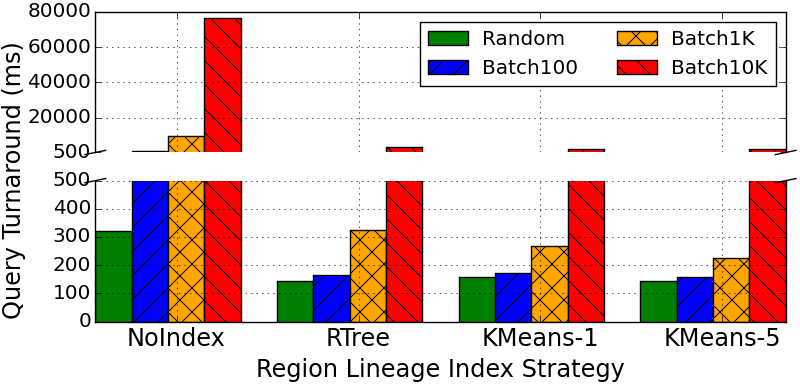
\includegraphics[width=85mm]{pictures/SIFTIndex-Time}
\caption {Runtime profile of the VOCSIFTFisher pipeline with four indexing strategies for region lineage.
    \label{fig:sift-time}
}
\end{center}
\end{figure}

\begin{figure}[h]
\begin{center}
    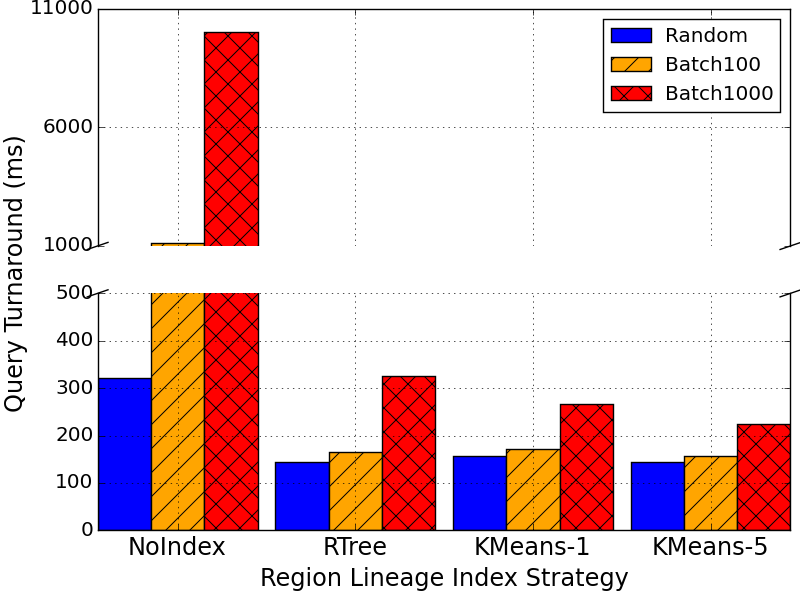
\includegraphics[width=85mm]{pictures/SIFTQuery-Time}
\caption {Query performance profile of the SIFTExtractor transformer in VOCSIFTFisher pipeline with four indexing strategies for region lineage in log scale
    \label{fig:sift-query}
}
\end{center}
\end{figure}

\subsection{End-to-end Pipeline Performance}

\begin{table}[ht]
\begin{center}
    \caption{Overhead Profile of Gineala on the VOCSIFTFisher, SourceExtractor, and MNIST Pipelines}
    \begin{scriptsize}
    \begin{tabular}{ | p{1.5cm} | p{2cm} | p{2cm} | p{1.5cm} | }
    \hline
    Pipeline & VOCSIFTFisher & SourceExtractor & MNIST  \\ \hline \hline
    Baseline & 780.8s & 279.7s & 56.4s \\ \hline
    Slowdown & 38.4\% & 25.6\% & 62.2\%   \\ \hline
    Memory & 38.5\% & 43.7\% & 200\%\\ \hline
    Meta Space & 109.9~GB & 204.4~MB & 78.9~MB \\ \hline
    Data Space & 615.7~GB & 506.9~GB & 11.8~GB\\ \hline
    \end{tabular}
    \end{scriptsize}
    \label{tb:apps-overhead}
\end{center}   
\end{table}

\subsection{Scalability}
Figure~\ref{fig:scalability}. Scalability shown on 8, 16, 32, 64 nodes.

\begin{figure}[h]
\begin{center}
    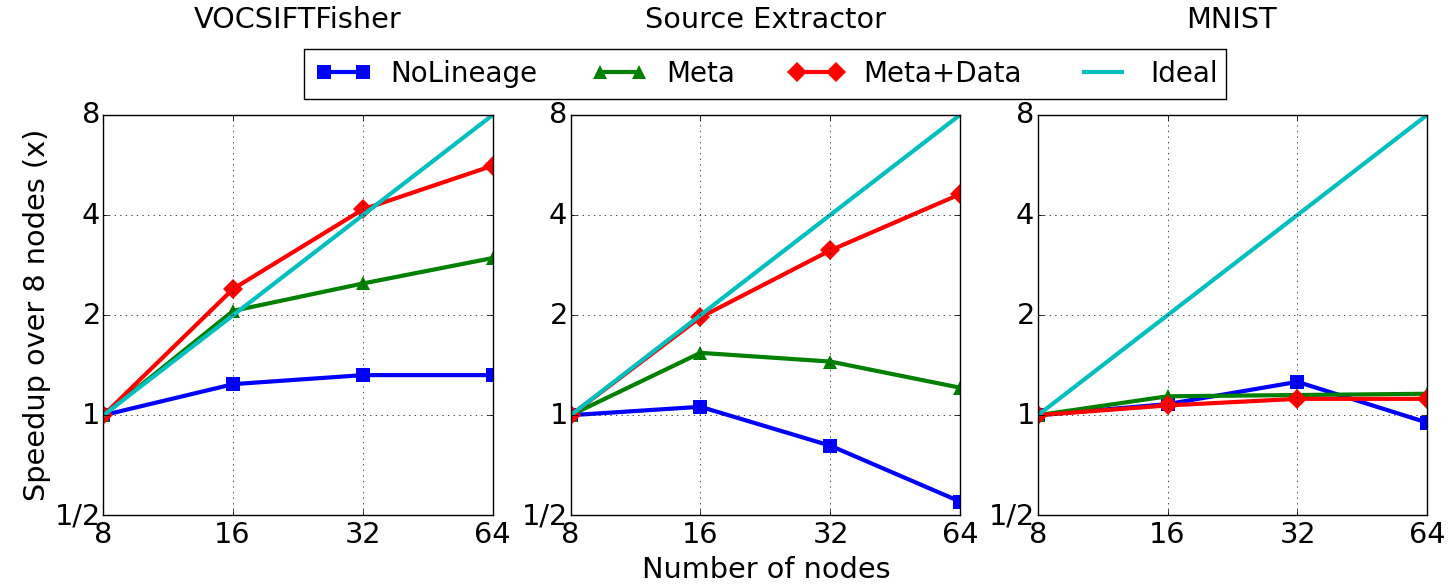
\includegraphics[width=85mm]{pictures/Scalability}
\caption {Relative Speedup of the VOCSIFTFisher, Source Extractor, and MNIST Pipelines with Gineala over Eight Nodes.
    \label{fig:scalability}
}
\end{center}
\end{figure}

\subsection{Use Case}
Query-oriented instrumentation, collect slowdown, and query performance.

\section{Related Work}
\label{sec:Related}
Lineage capturing and query systems have been proposed for RDMBS~\cite{widom04}, array-based
DBMS~\cite{wu13}, MapReduce frameworks~\cite{ikeda11, logothetis13}, and Linux operating system~\cite{devecsery14}.


\section{Conclusion and Future Work}
\label{sec:Conclusion}
Conclusion

%ACKNOWLEDGMENTS are optional
\section{Acknowledgments}
This research is supported in part by NSF CISE Expeditions Award CCF-1139158, LBNL Award 7076018, and DARPA XData Award FA8750-12-2-0331, and gifts from Amazon Web Services, Google, SAP,  The Thomas and Stacey Siebel Foundation, Adatao, Adobe, Apple, Inc., Blue Goji, Bosch, C3Energy, Cisco, Cray, Cloudera, EMC, Ericsson, Facebook, Guavus, Huawei, Intel, Microsoft, NetApp, Pivotal, Samsung, Splunk, Virdata, VMware, and Yahoo!. 

%
% The following two commands are all you need in the
% initial runs of your .tex file to
% produce the bibliography for the citations in your paper.
\bibliographystyle{abbrv}
\bibliography{Lineage} % sigproc.bib is the name of the Bibliography in this case
% You must have a proper ".bib" file
%  and remember to run:
% latex bibtex latex latex
% to resolve all references
%
% ACM needs 'a single self-contained file'!
%
%APPENDICES are optional
%\balancecolumns



\balancecolumns

% That's all folks!
\end{document}
